\documentclass{beamer}
\usepackage[utf8]{inputenc}
\usepackage[brazil]{babel}
\usetheme{Warsaw}

\title{Analisando Composições de Serviços com Apache Hadoop}
\subtitle{Coreografia \emph{versus} Orquestração}
\author{Carlos Eduardo M. Santos, Thiago Furtado}\institute{Universidade de São Paulo - IME\\MAC0431 - Introdução à Computação Paralela e Distribuída}
\date{19 de outubro de 2012}

\begin{document}

\begin{frame}
\titlepage
\end{frame}

\section{Introdução}

\begin{frame}
É fácil analisar o tempo de resposta do serviço chamado diretamente.
\begin{figure}
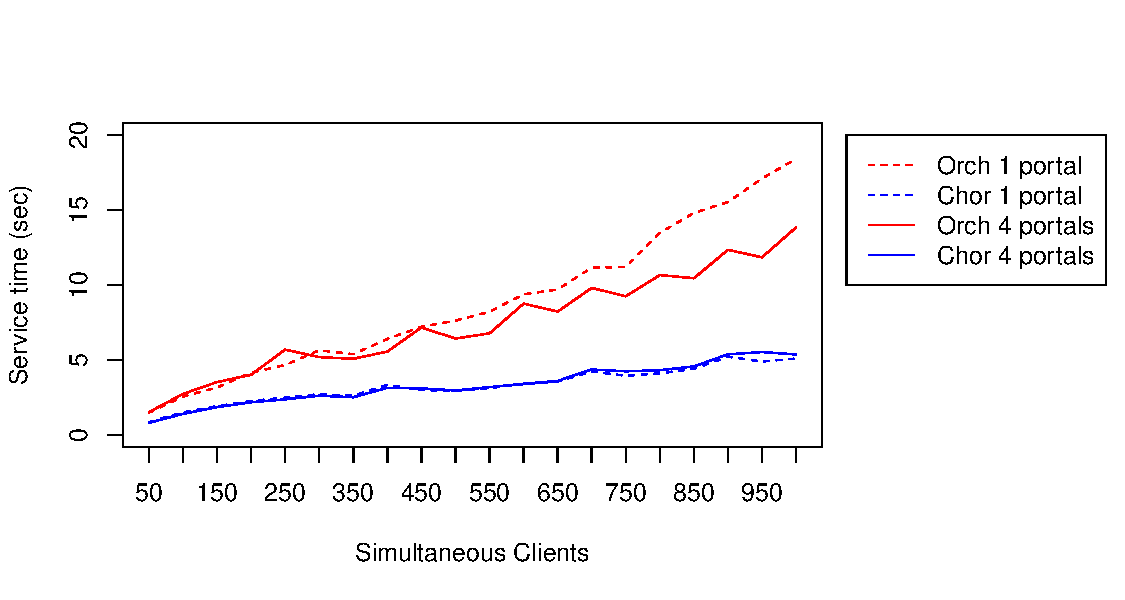
\includegraphics[width=\linewidth,clip=true,trim=1mm 2mm 3mm 20mm]{figures/portals1-4}
\caption{Chamadas a operações do serviço \emph{Portal}.}
\end{figure}
\end{frame}

\begin{frame}
Mas e dos outros serviços participantes da composição?
\begin{figure}
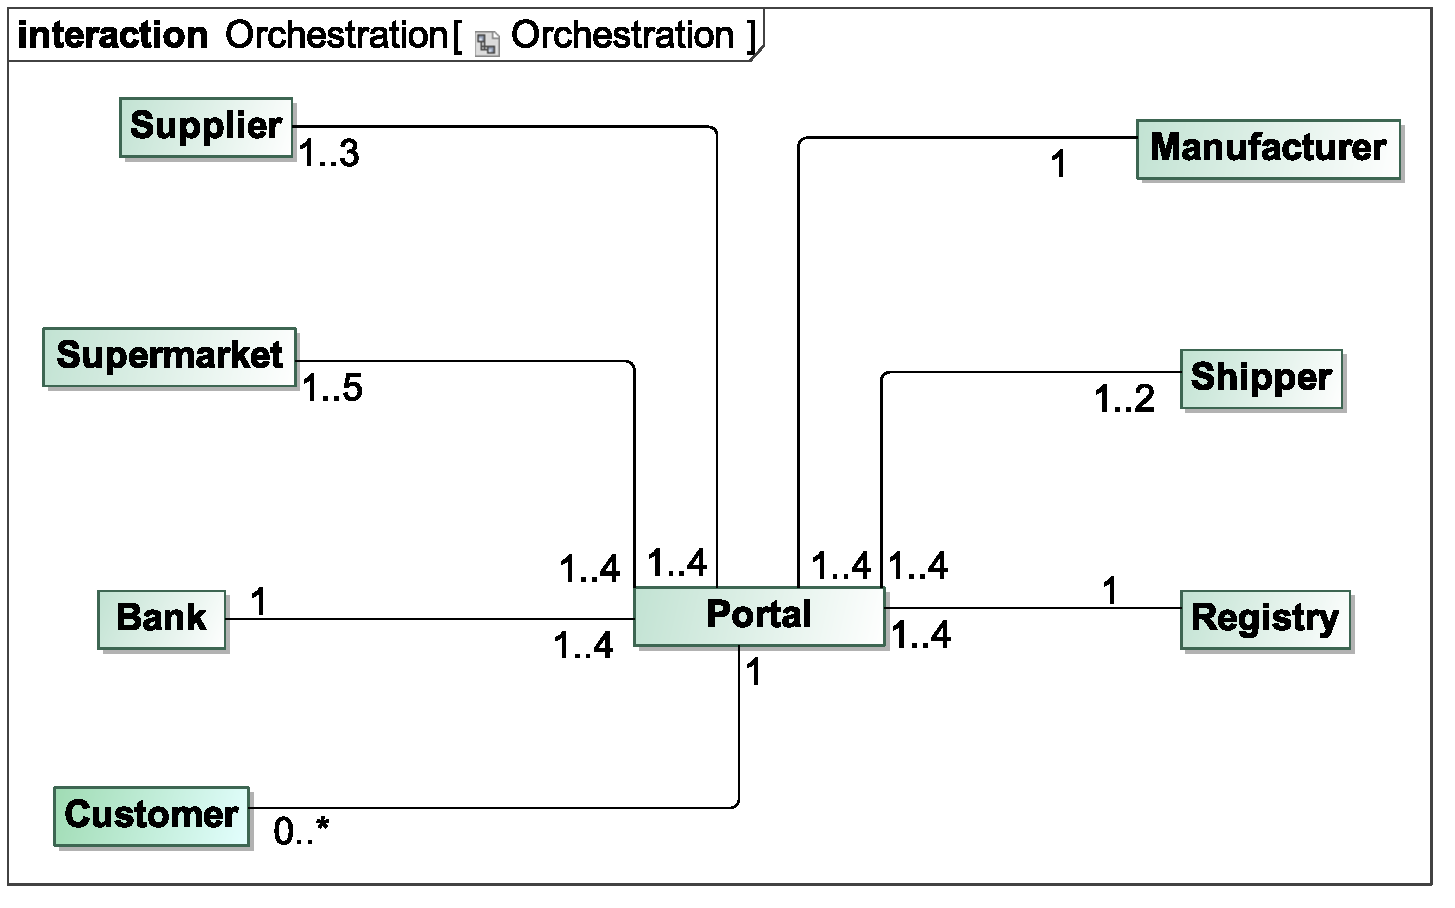
\includegraphics[width=\textwidth,clip=true,trim=7mm 9mm 8mm 16mm]{figures/orch}
\caption{Interação entre serviços na versão orquestrada.}
\end{figure}
\end{frame}

\begin{frame}
\begin{figure}
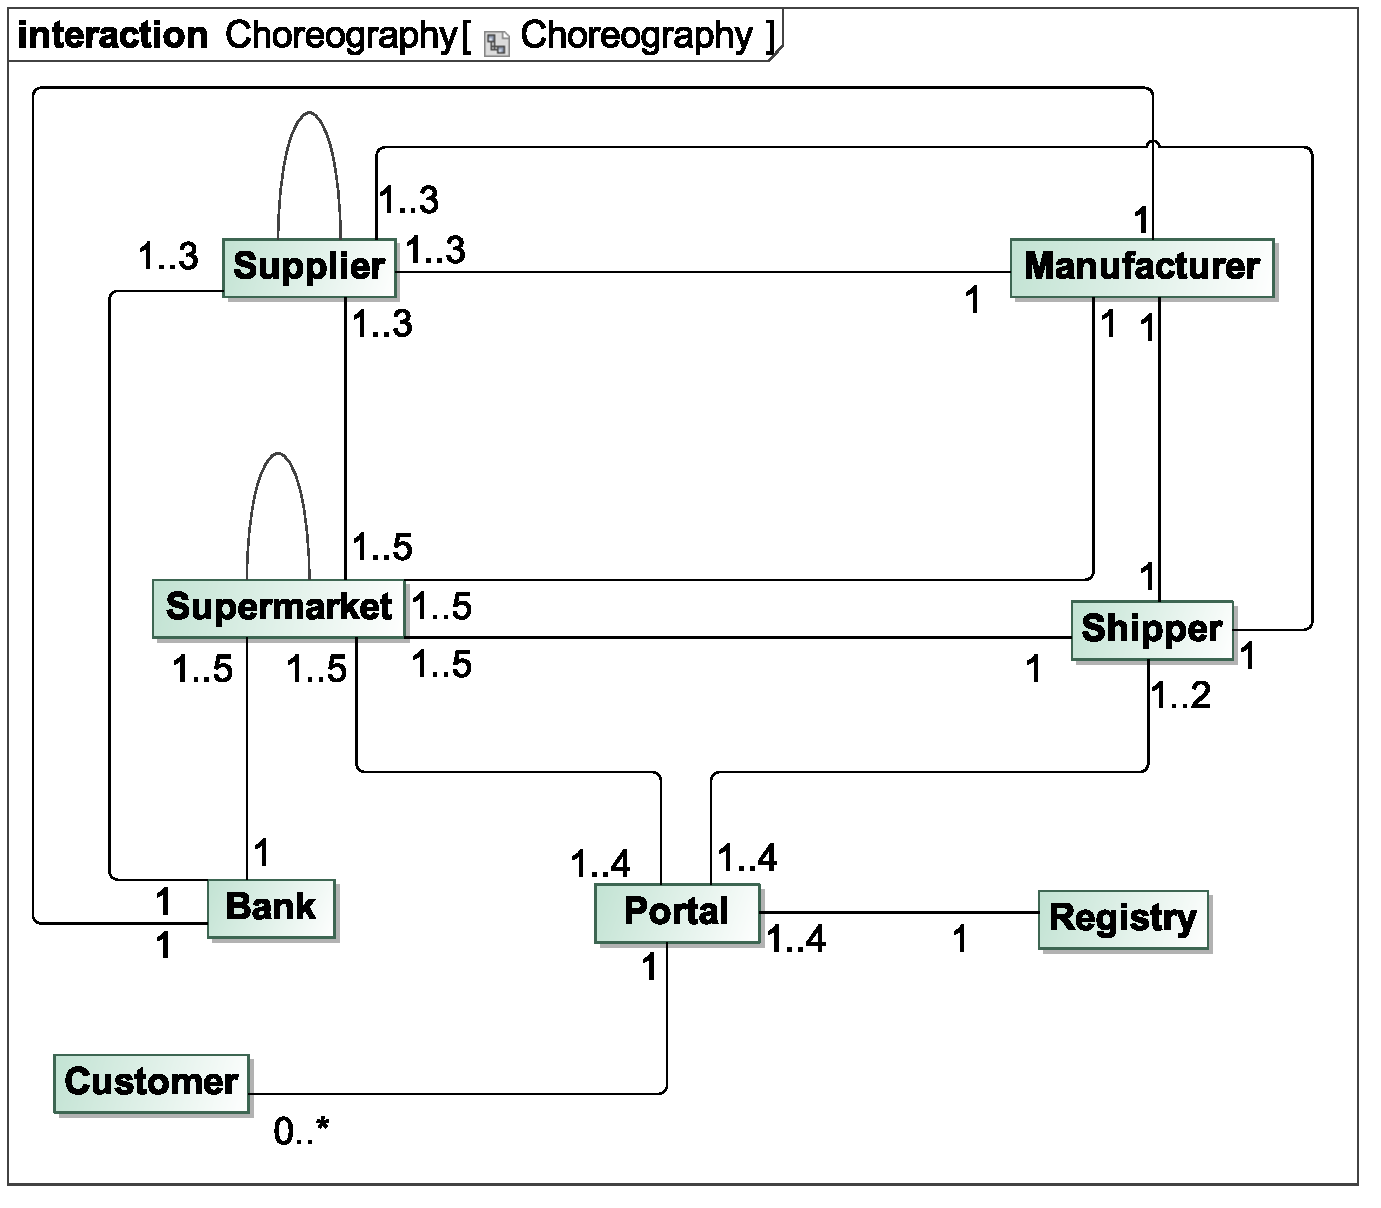
\includegraphics[height=0.85\textheight,clip=true,trim=2mm 10mm 5mm 14mm]{figures/chor}
\caption{Interação entre serviços na versão coreografada.}
\end{figure}
\end{frame}

\begin{frame}
\begin{itemize}
  \item Gerar carga em um serviço por vez?
  \begin{itemize}
    \item Dependências entre serviços;
    \item Muitos estados, entradas e saídas possíveis;
    \item Outros serviços numa mesma máquina;
  \end{itemize}
  \item Analizar o log dos servidores:
  \begin{itemize}
    \item Sem necessidade de realizar outros testes;
    \item Permite comparar com o resultado de toda a composição;
    \item Problemas? Logs: tamanho, formato.
  \end{itemize}
\end{itemize}
\end{frame}

\section{Dados}

\subsection{Gerador de Carga}
\begin{frame}[fragile]
Saída do gerador de carga (125 MB):

\begin{verbatim}
# orch,1,50,1349926295888
424
892
(...)
2017
2038
# orch,1,100,1349926297945
1110
1189
(...)
\end{verbatim}

\begin{description}
\item[orch,1] Arquitetura
\item[50/100] Número de clientes simultâneos (eixo x)
\item[134552629...] Tempo em milissegundos
\end{description}
\end{frame}

\subsection{Log}
\begin{frame}[fragile]
Formato modificado do log de Apache Tomcat (200 GB):
\begin{verbatim}
198.55.32.149 - - [09/Oct/2012:02:47:56 -0700] "POST
/supermarket5/orchestration HTTP/1.1" 200 914 811
\end{verbatim}
A qual teste esse acesso pertence?
\end{frame}

\section{Hadoop}
\subsection{Map}
\begin{frame}[fragile]
Pré-requisito: pela saída do gerador de carga, gerar uma tabela de horários e parâmetros dos testes. Utilizando-a, podemos obter \emph{orch,1,50} através de \emph{10/Oct/2012:20:31:35}.

\begin{verbatim}
MAP
while has line
    time <- get_time(line)
    params <- get_params(time)
    if params is not empty
        output(params, time)
\end{verbatim}
\end{frame}

\subsection{Reduce}
\begin{frame}[fragile]
Para cada conjunto de parâmetros (arquitetura, teste), as médias e seus intervalos de confiança serão mostrados em gráficos.

\begin{verbatim}
REDUCE
while has value
    values.store(value)
mean <- get_mean(values)
ic <- get_ic(values, mean)
output(key, "mean,ic")
\end{verbatim}
\end{frame}

\subsection{Cuidados}
\begin{frame}
Alguns cuidados são necessários nos cálculos da redução:
\begin{itemize}
\item \emph{Overflow} numérico
\item \emph{Overflow} de memória
\end{itemize}
\end{frame}

\begin{frame}
Dúvidas?
\end{frame}

\end{document}
